%%%%%%%%%%%%%%%%%%%%%%%%%
% PACKAGES              %
%%%%%%%%%%%%%%%%%%%%%%%%%
\documentclass{report} % book|article|…

\usepackage[utf8x]{inputenc}    % accents
\usepackage{geometry}           % marges
\usepackage[english]{babel}     % langue
\usepackage{graphicx}           % images
\usepackage{verbatim}           % texte préformaté
\usepackage{fancyhdr}           % fancy
\usepackage{filecontents}       % write file directly
\usepackage{csvsimple}          % csv reader
\usepackage{lastpage}	        % get number of last page
\usepackage{listings}           % source code 
\usepackage{url}                % clickable urls 
\usepackage{hyperref}           % href urls 
\usepackage{float}              % exact placement of figures 
\usepackage{longtable}          % tables splitted on multiple pages
\usepackage{booktabs}           % hrules on splitted tables
\usepackage{multicol}           % multicolumn
\usepackage{caption}            % put easily captions on non figure objects

% packages for graphics
\usepackage{fancybox}         
\usepackage{pgfplots}        
\usepackage{pgfplotstable}
\usepgfplotslibrary{dateplot}




%%%%%%%%%%%%%%%%%%%%%%%%%
% PRÉAMBULE             %
%%%%%%%%%%%%%%%%%%%%%%%%%
\title{CBD project report} 
\author{Lucas Bourneuf}
% laisser vide pour date de compilation
\date{} 

% FORMAT PAGES         
\pagestyle{fancy} % nom du rendu (définit les lignes suivantes)
        \lhead{} % left head
        \chead{CBD report} % center head
        \rhead{} % right head
        \lfoot{} % left foot
        \cfoot{\thepage/\pageref{LastPage}} % center foot
        \rfoot{} % right foot


% Definitions necessary for print bar plots
\pgfplotstableread[col sep=comma]{data/hepcidinBackgroundQuantification.csv}\dataHepBackQuantif
\makeatletter
\pgfplotsset{
    /pgfplots/flexible xticklabels from table/.code n args={3}{%
            \pgfplotstableread[#3]{#1}\coordinate@table
            \pgfplotstablegetcolumn{#2}\of{\coordinate@table}\to\pgfplots@xticklabels
            \let\pgfplots@xticklabel=\pgfplots@user@ticklabel@list@x
        }
}
\makeatother




%%%%%%%%%%%%%%%%%%%%%%%%%
% BEGIN                 %
%%%%%%%%%%%%%%%%%%%%%%%%%
\begin{document}
        \renewcommand*\thesection{\arabic{section}} % no chapter numerotation
        \maketitle % page de titre




%%%%%%%%%%%%%%%%%%%%%%%%%
% SECTION               %
%%%%%%%%%%%%%%%%%%%%%%%%%
\section*{Introduction}
    \paragraph*{}
    Here is the report of a Database project that involve an hepcidin csv database parsing, a SQL database creation, and some requests on it + data generation.\\
    In the next pages, technologies, tools, architecture and results will be quickly presented.
    \paragraph*{}
    Goal was to transform a csv database into sql database, and finally extract some data about \textsc{Hepcidin}, the protein mainly concerned by csv database.


%%%%%%%%%%%%%%%%%%%%%%%%%
% SECTION               %
%%%%%%%%%%%%%%%%%%%%%%%%%
\section{Technologies}
    \paragraph*{}
    Here a non-exhaustive list of tools that have a place in this project.
    Some tools, like ORMs\footnote{\href{http://www.sqlalchemy.org/}{SQLAlchemy} for example}, haven't been used,
    for conserve a project very close to SQL management, as requested by specifications.
    \begin{description}
            \item[Python 3] main program and scripting around databases;
            \item[sqllite] database creation, hosting, querying;
            \item[networkx] graph generation;
            \item[matplotlib] graph printing;
            \item[pylint] for code review;
            %\item[] ;
            %\item[] ;
            %\item[] ;
    \end{description}
    The website \url{http://ondras.zarovi.cz/sql/demo/} was used for generation of EAM drawing.
    \paragraph*{}
    Moreover, a quick treatment was primarily applied to all provided events data :
\begin{lstlisting}[language=bash]
sed -i 's/\\"//g' data_hepcidin/events_*
\end{lstlisting}
    \paragraph*{}
    Its necessary for conserve a perfect alignment in the csv files.
    For avoid this problem in generated files, separator character will be commas.



%%%%%%%%%%%%%%%%%%%%%%%%%
% SECTION               %
%%%%%%%%%%%%%%%%%%%%%%%%%
\newpage
\section{Architecture}
        \paragraph*{}
        The code architecture is very simple and follow \textbf{some} conventions of the PEP 8.
        \begin{description}
                \item[database] a module that wraps database treatments. (ORM-like);
                \item[main] script of cbd package that use database and generate wanted data;
        \end{description}

        \paragraph*{}
        The important thing is the database itself, designed for reach the 4NF, with some exceptions : 
        for example, because of no real uniformicity of the csv database on \textit{edge labels}, there is no dedicated relation.
        The description of the model can be found in Figure~\ref{fig:mea}.
        \begin{center}
        \end{center}
        \begin{figure}[H] 
                \centering
                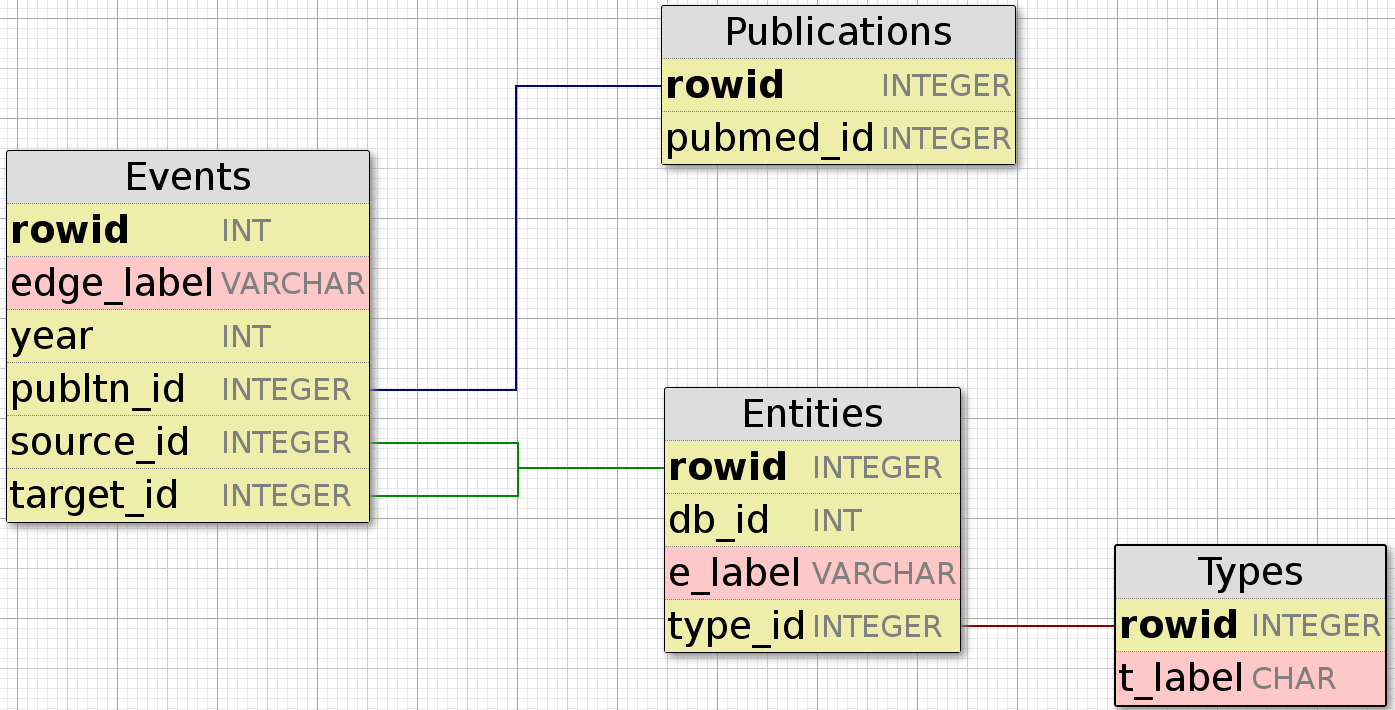
\includegraphics[width=1.0\textwidth]{images/MEA.png}
                \caption{Entity Association Model for the generated and used database}
                \label{fig:mea}
        \end{figure}      




%%%%%%%%%%%%%%%%%%%%%%%%%
% SECTION               %
%%%%%%%%%%%%%%%%%%%%%%%%%
\newpage
\section{First need}
    \paragraph*{}
    A quick overview of the data is necessary : Figure~\ref{fig:eventperyear} show number of events that involve hepcidin per year.
    \begin{figure}[H] 
      \centering
      \begin{tikzpicture}
          \begin{axis}[
                  %,no mark % retract marks at point location
                  ,xlabel={Year}
                  ,ylabel={Events}
                  ,grid=major % grid on all axis
                  ,axis lines=left
                  ,ymajorgrids
                  ,legend style={legend pos=north east}
              ]
              \addplot table [col sep=comma,x=year,y=eventCount] {data/interactionWithHepcidinByYear.csv};
              %\legend{Events}
          \end{axis}
      \end{tikzpicture}
      \caption{Events that involve Hepcidin for each considered year}
      \label{fig:eventperyear}
    \end{figure}




%%%%%%%%%%%%%%%%%%%%%%%%%
% SECTION               %
%%%%%%%%%%%%%%%%%%%%%%%%%
\newpage
\section{Second need}
        \paragraph*{}
        Hepcidin protein is associated with many diseases. For have the exact names of diseases associated with hepcidin per year, 
        look at file \textsc{data/hepcidinDiseaseAssociation.csv}. The Figure~\ref{fig:diseasePerYear} show numbers of diseases.
        \begin{figure}[H] 
                \centering
                \begin{tikzpicture}
                  \begin{axis}[
                          %,no mark % retract marks at point location
                          ,xlabel={Year}
                          ,ylabel={Diseases}
                          ,grid=major % grid on all axis
                          ,axis lines=left
                          ,ymajorgrids
                          ,legend style={legend pos=north east}
                      ]
                      \addplot table [col sep=comma,x=year,y=diseases] {data/hepcidinDiseaseAssociationCount.csv};
                      %\legend{Events}
                  \end{axis}
                \end{tikzpicture}
                \caption{Count of diseases that are targeted by Hepcidin for each considered year}
                \label{fig:diseasePerYear}
        \end{figure}




%%%%%%%%%%%%%%%%%%%%%%%%%
% SECTION               %
%%%%%%%%%%%%%%%%%%%%%%%%%
\newpage
\section{Third and fourth need}
        \paragraph*{}
        An important notion is the \textbf{Background event}. An event is said background when it appears many times in different years.
        There is some things we can show about these particular events. \\
        First, we can isolate all protein that are related to hepcidin with at least two occurence. This big table is shown in 
        appendix at the end of this report.
        \paragraph*{}
        The Figure~\ref{fig:backgroundQuantification} shows the quantity of events that involves proteins and hepcidin, compared 
        to the number of background events.\\
        \begin{figure}[H] 
                \centering
                \begin{tikzpicture}
                        \begin{axis}[        
                                ybar, ymin=0,
                                xlabel=Associations,
                                ylabel=Count of association,
                                flexible xticklabels from table={data/hepcidinBackgroundQuantification.csv}{association}{col sep=comma},
                                xticklabel style={text height=1.5ex}, % To make sure the text labels are nicely aligned
                                xtick=data,
                                nodes near coords,
                                nodes near coords align={vertical}
                        ]
                        \addplot[green!20!black,fill=green!50!white] table [col sep=comma,x=association,y=count,x expr=\coordindex] {data/hepcidinBackgroundQuantification.csv};
                        \end{axis}
                \end{tikzpicture}
                \caption{Comparison of background events quantity and events quantity}
                \label{fig:backgroundQuantification}
        \end{figure}



%%%%%%%%%%%%%%%%%%%%%%%%%
% SECTION               %
%%%%%%%%%%%%%%%%%%%%%%%%%
\newpage
\section{Fifth need}
        \paragraph*{}
        With the help of \href{http://matplotlib.org/}{\textit{matplotlib}} and \href{https://networkx.github.io/}{\textit{networkx}},
        Many graphs of interactions can be draw. For each year, two graph are performed : one that show only the background events, 
        and another one that show only the unique events.
        \paragraph*{}
        Some interesting graphs are shown there. All can be regenerated and available in outputs directory (default is \textsc{data/outputs/})
        \paragraph*{}
        These follow always the same color convention : the more publications describes an interaction, the deeper is the edge color.
        For example, in Figure~\ref{fig:interact2001NOBK}, hepcidin and IRPS proteins interaction seems to be described in more publications than the others.
        \paragraph*{}
        Another interesting thing is the Figure~\ref{fig:interact2001NOBK} that show that all protein interaction with hepcidin found in 2001 
        are considered like background. (because of no unique interaction)\\
        All these background interactions are show in Figure~\ref{fig:interact2001BACK}.
        \paragraph*{}
        Two gif files are available for simplify watching of these graphs.
        They can be generated with \textit{ImageMagick} with a simple script like :
\begin{lstlisting}[language=bash]
convert -delay 1000 -loop 1 hepcidinGraphInteractionsBack*.png backgroundInteractions.gif
convert -delay 1000 -loop 1 hepcidinGraphInteractionsNonBack*.png nonBackgroundInteractions.gif
\end{lstlisting}
        \begin{figure}[H] 
                \centering
                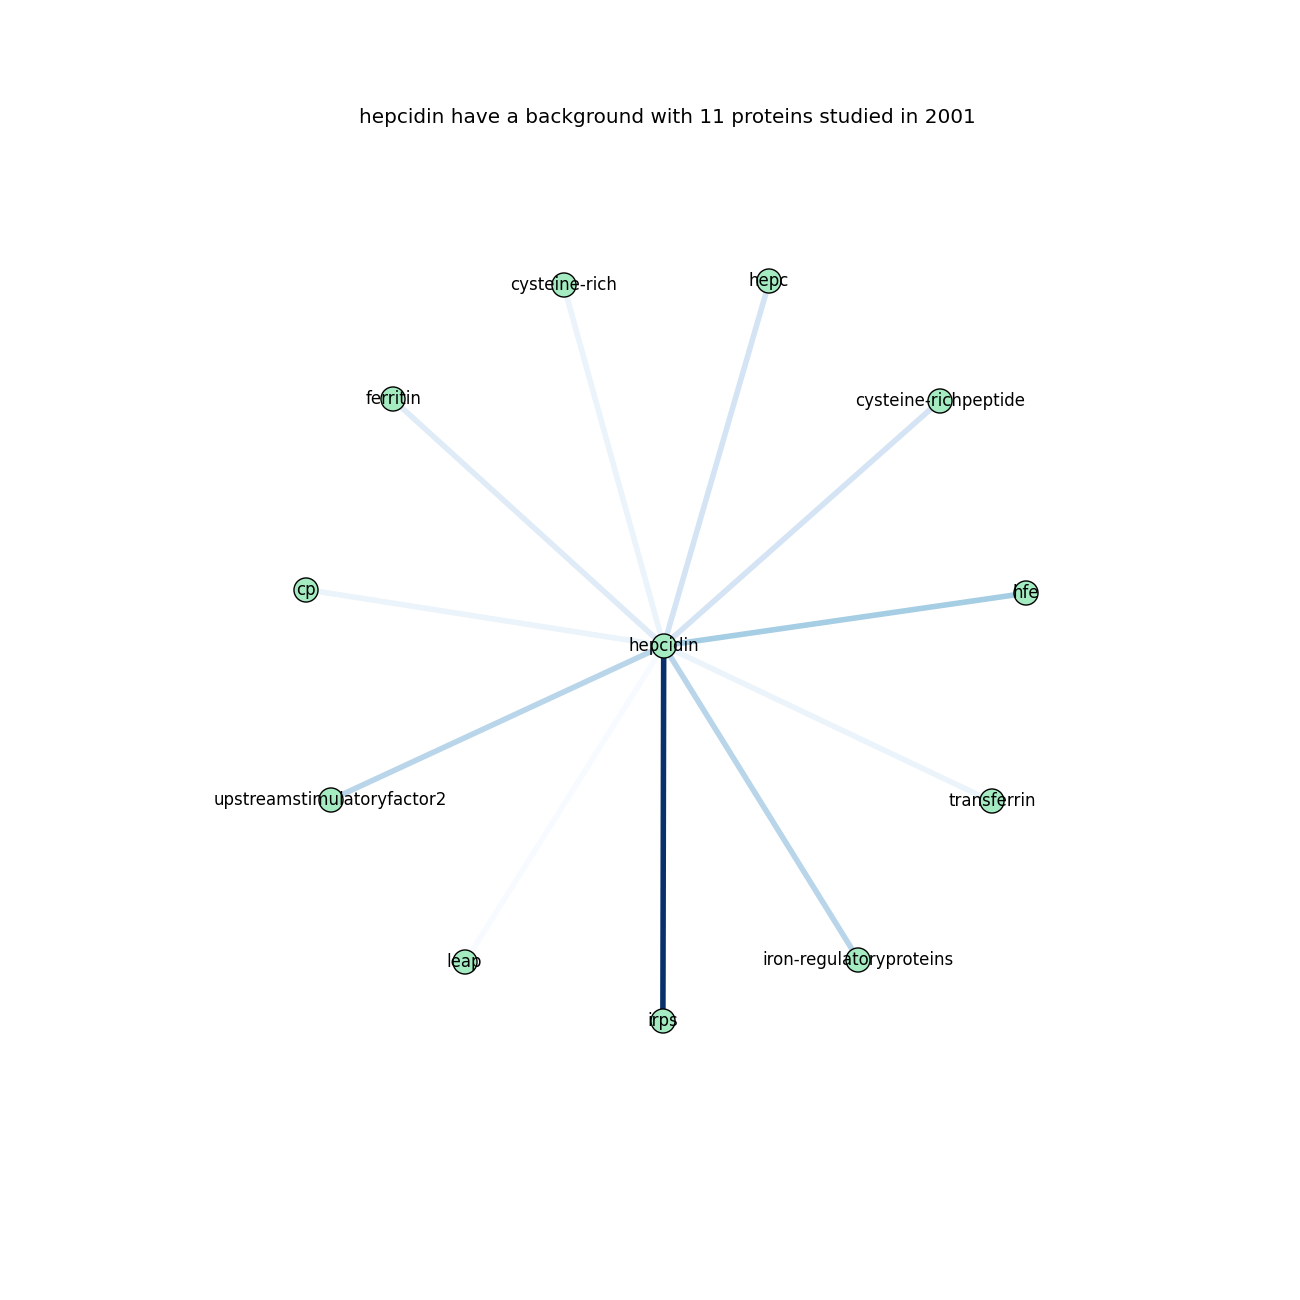
\includegraphics[width=1.0\textwidth]{images/hepcidinGraphInteractionsBackground2001.png}
                \caption{Background interaction graph of hepcidin (center) with other protein in 2001.}
                \label{fig:interact2001BACK}
        \end{figure}
        \begin{figure}[H] 
                \centering
                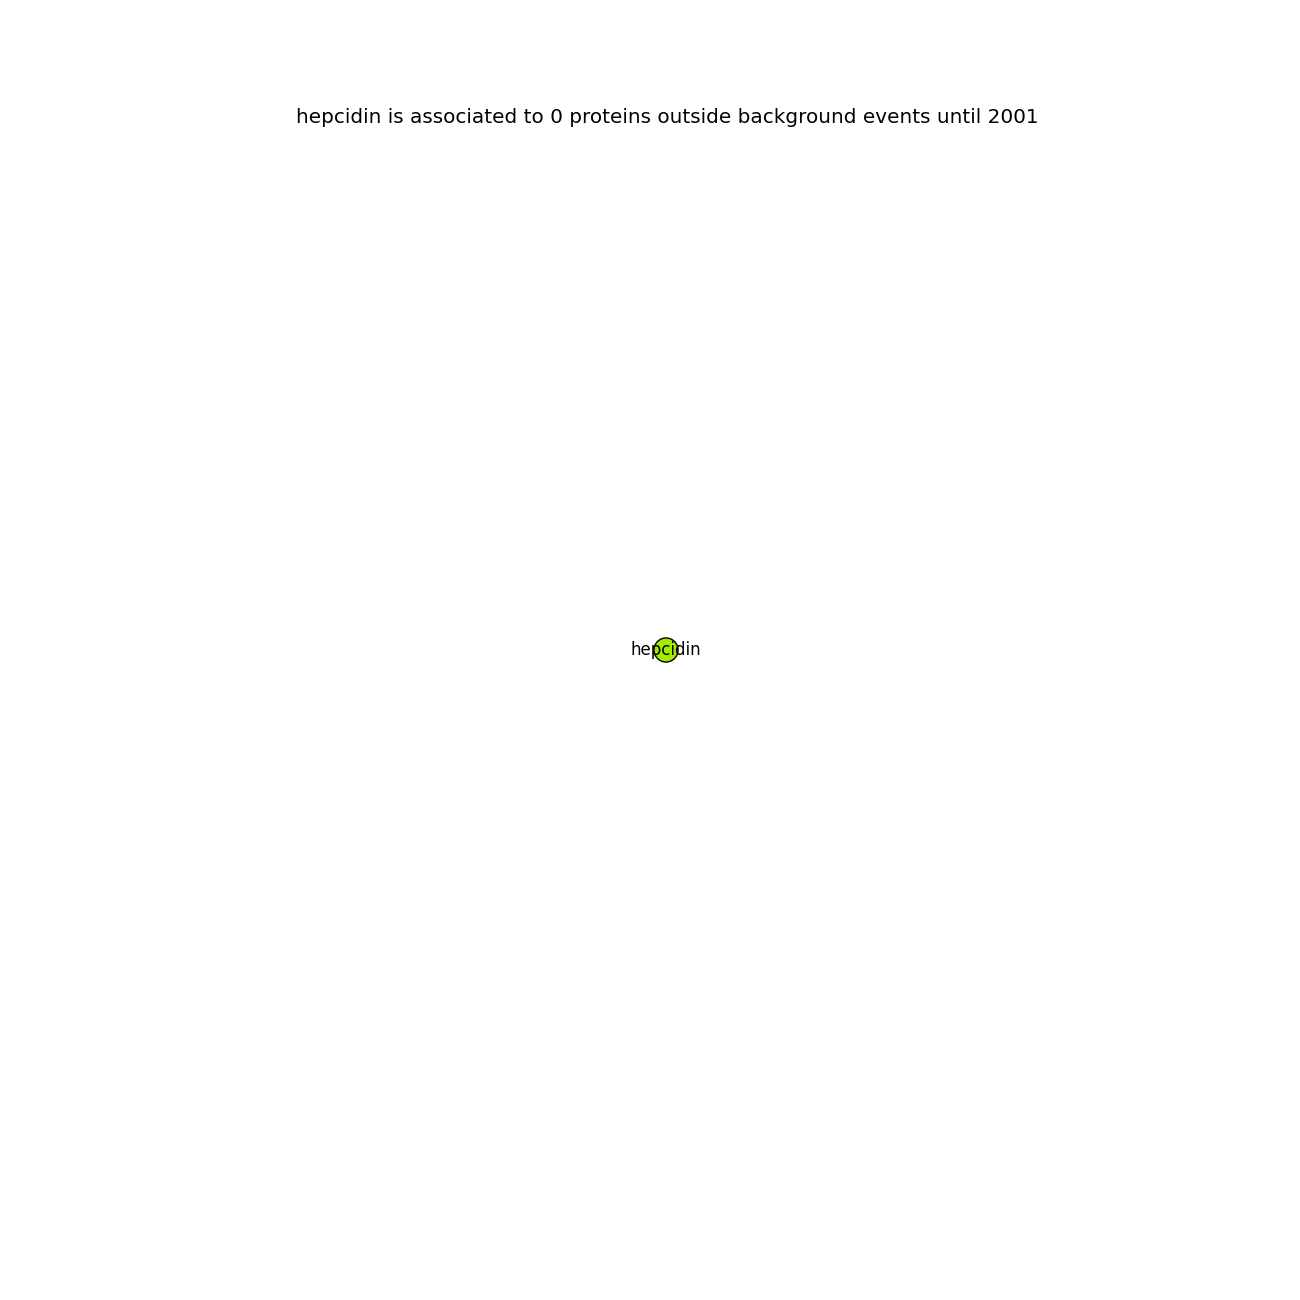
\includegraphics[width=1.0\textwidth]{images/hepcidinGraphInteractionsNonBackground2001.png}
                \caption{Non Background Interaction graph of hepcidin (center) with other protein in 2001.}
                \label{fig:interact2001NOBK}
        \end{figure}
        \begin{figure}[H] 
                \centering
                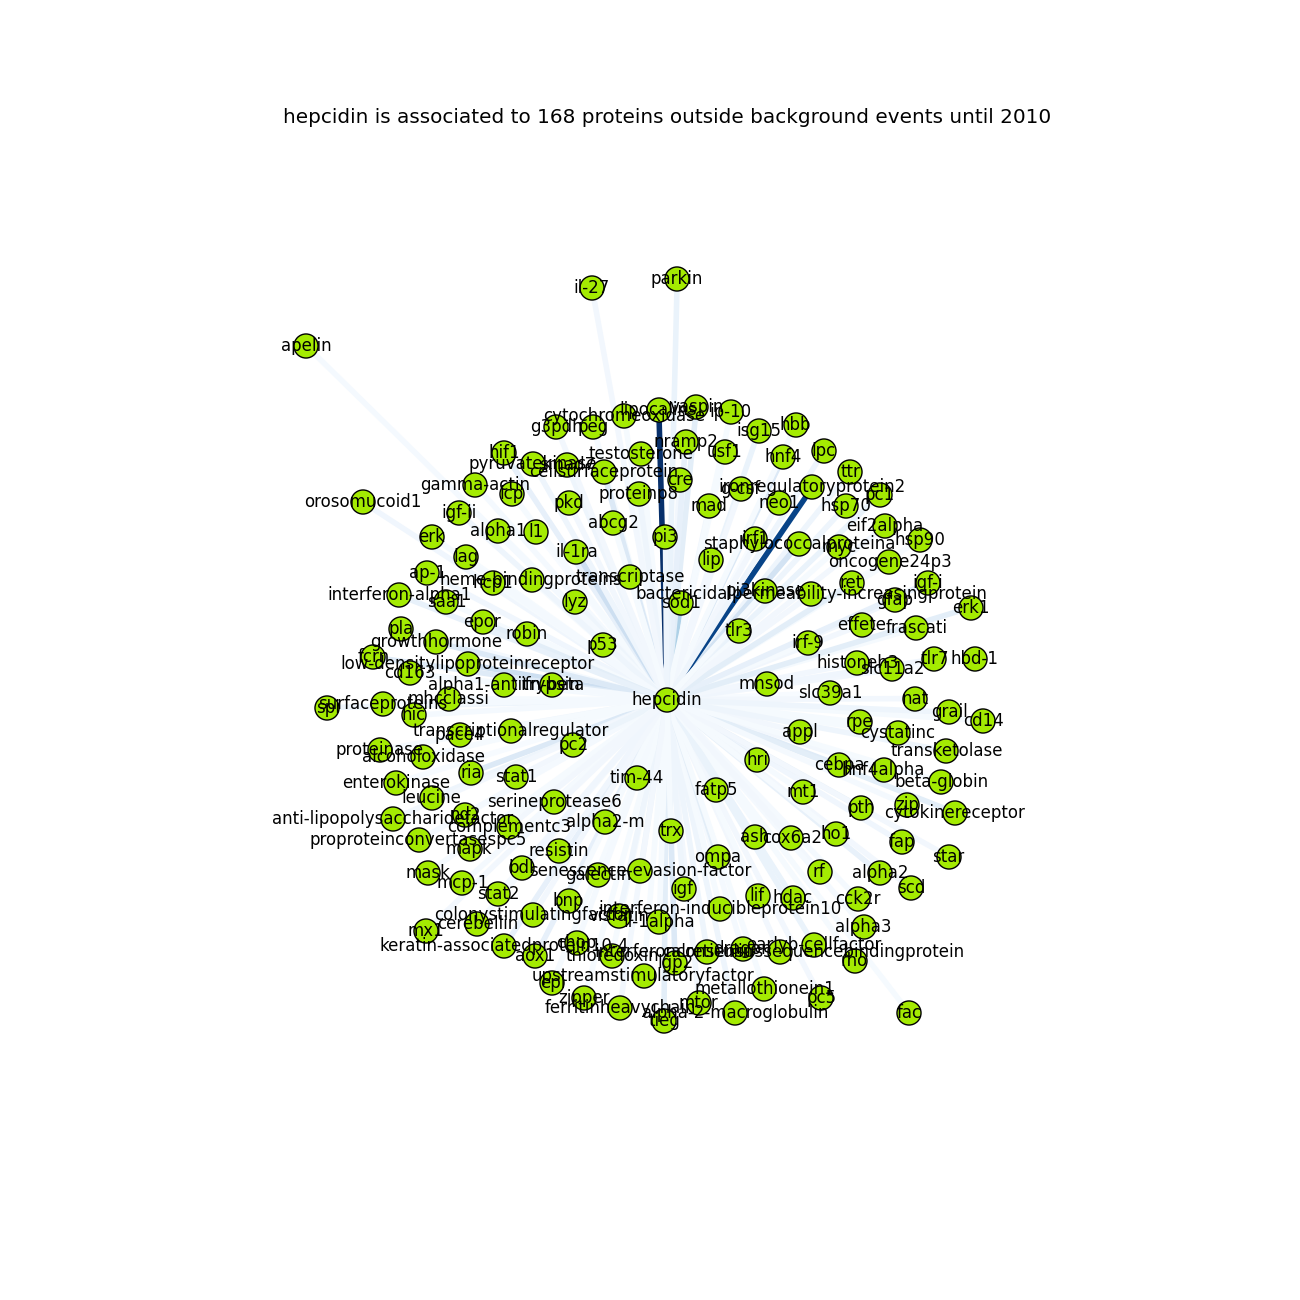
\includegraphics[width=1.0\textwidth]{images/hepcidinGraphInteractionsNonBackground2010.png}
                \caption{Non Background Interaction graph of hepcidin (center) with other protein in 2010.}
                \label{fig:interact2010NOBK}
        \end{figure}



%%%%%%%%%%%%%%%%%%%%%%%%%
% APPENDICES            %
%%%%%%%%%%%%%%%%%%%%%%%%%
\newpage
\begin{appendix}
\section{Appendix}

        \pgfplotstableset{
                begin table=\begin{longtable},
                end table=\end{longtable},
        }
        \pgfplotstabletypeset[
            col sep=comma,
            header=true,
            columns={protein,yearsCount},
            string type,
            columns/protein/.style={column name=Protein, column type=l},
            columns/yearsCount/.style={column name=Number of occurences, column type=c},
            every head row/.style={before row=\toprule, after row=\midrule\endhead}, % repeat header on the top
            every last row/.style={after row=\bottomrule}
        ]{data/hepcidinBackgroundEvents.csv}
        \begin{center}
                \textsc{Proteins related to Hepcidin in a background event}
        \end{center}



\end{appendix}
\end{document}
% END



